\section{History and Theory}

Cosmic rays were discovered in 1911 by Victor Hess, for which he shared the 1936 Nobel Prize \cite{pleijel1936hessnobel}. Since his discovery, experiments have been conducted to determine the energy spectrum, arrival directions, and composition of cosmic rays.  The University of Utah has historically been involved in this research because of its proximity to the high deserts of the Great Basin. Among other things, the region has low light pollution and minimal cloud cover. Utah's experiments have primarily relied on the detection of nitrogen fluorescence with arrays of wide-angle telescopes. Two such experiments, Fly's Eye and High Resolution Fly's Eye (HiRes), were  instrumental in improving resolution at the high end of the energy spectrum \cite{abuzayyad2000hires, bird1994flyseye}. In 2007, HiRes was superseded by the Telescope Array Project, an international collaboration between the University of Utah, the University of Tokyo, and others. Telescope Array improves on the accuracy of HiRes by adding an array of ground-based scintillators \cite{stratton2012ta}.

It has been determined that most cosmic rays are hydrogen nuclei, with a small fraction of heavier nuclei like iron. It has also been found that energies obey a decreasing power law. In 1966, a theoretical maximum energy of \SI{5e19}{eV} was conjectured, leading to interest in the highest energy events \cite{greisen1966cutoff, zatsepin1966cutoff}. This theoretical maximum energy is known as the GZK cutoff, and results from the interaction of cosmic rays with the cosmic microwave background. The primary pathways are
\begin{equation}
\begin{aligned}
    \gamma + p &\rightarrow \Delta^+ \rightarrow p + \pi^0 \\
    \gamma + p &\rightarrow \Delta^+ \rightarrow n + \pi^+.
\end{aligned}
\end{equation}
In these interactions, a proton collides with a background photon, leading to the loss of energy through a $\pi^0$ or $\pi^+$. Over large distances, this and similar processes gradually reduce the energy of the proton to less than the threshold for the interaction. Interestingly, HiRes and other experiments have confirmed that the energy spectrum continues past the GZK cutoff. One of the primary goals of the Telescope Array project is determining the source of particles at this tail end of the spectrum. Below \SI{e18}{eV}, cosmic rays are believed to be of galactic origin and accelerated by supernova shock fronts \cite{abuzayyad2000hires}. Above this, one can only make educated guesses. If particles are contained by a magnetic field during their acceleration, there are restrictions on the size and field strength of accelerators. These restrictions can be summarized in a Hillas Plot, shown in Figure \ref{fig:hillas}. 

The decreasing power law of cosmic ray flux creates a problem for high energy experiments. The flux in this regime is very low (on the order of one per square kilometer per century), so direct detection is impractical. Fortunately, ultra high energy rays interact with the atmosphere and can be indirectly observed by distant detectors. High energy cosmic rays initiate a cascade of photons and charged particles (mostly fermions) upon entering the atmosphere. This shower multiplies through an alternating sequence of Bremsstrahlung and pair creation \cite{abuzayyad2000hires}. Shower particles interact with atmospheric nitrogen, producing fluorescence which can be observed by a sensitive detector. The slant depth of the fluorescence peak increases with the energy of the primary, with ultra high energy cascades typically peaking between \num{725} and \SI{890}{g/cm^2} \cite{abuzayyad2000hires}. The Great Basin, at a depth of roughly \SI{860}{g/cm^2}, is ideally situated to view these events.

\begin{figure}[ht]
    \label{fig:hillas}
    \centering
    \includegraphics[width=0.8\textwidth]{HillasPlot}
    \caption{A Hillas Plot, taken from Yoshida \cite{yoshida1998uhecr}. Structures of larger size and stronger magnetic field can accelerate particles to higher energies. Candidates for the acceleration of \SI{e20}{eV} protons are radio galaxy lobes and active galactic nuclei.}
\end{figure}

Although cascades' individual particle interactions are well understood, their overall development and light production are too complex to be derived analytically. This precludes the possibility of directly determining properties of a cosmic ray from its cascade's light production. Simulated values and phenomenological models are used in place of analytic methods. A 1977 paper proposed a parameterization for the number of particles in a shower as a function of atmospheric depth, $X$ \cite{gaisser1977profile}. This parameterization, the Gaisser-Hillas profile, has become a standard in cosmic ray physics.
\begin{equation} \label{eq:gaisser_hillas}
    N(X) = N_\text{max} \left(\frac{X - X_0}{X_\text{max} - X_0}\right)
        ^{\frac{X_\text{max} - X_0}{\lambda}} 
        \exp{\left(\frac{X_\text{max} - X}{\lambda}\right)}
\end{equation}
$N_\text{max}$ is the maximum size of the shower, $X_0$ the depth of the first interaction, and $X_\text{max}$ the depth of the shower maximum. $\lambda$ is a scaling factor usually taken as $\SI{70}{g/cm^2}$. $N_\text{max}$, $X_0$, and $X_\text{max}$ depend straightforwardly on the energy of the primary particle (see Section \ref{sec:shower_gen}). In addition to knowing the number of particles in a shower, it is valuable to know distributions of their properties. CORSIKA simulates the interactions within a shower and records particle energies and velocities at each step \cite{heck1998corsika}. Various models of the CORSIKA data have been made, and are used with the Gaisser-Hillas profile to understand average particle behavior. For instance, Nerling gives a parameterization of the distribution of electron energies as a function of shower age \cite{nerling2006electron}.

Such models are useful when simulating shower light production. There are two main emission mechanisms. The first, fluorescence, occurs when shower particles excite atmospheric nitrogen. This emission is isotropic and heaviest in the UV. A parameterization of fluorescence production is given by Kakimoto as a function of the shower's atmospheric energy deposit \cite{kakimoto1996yield}. The second emission mechanism, Cherenkov radiation, can be thought of as a ``shock front'' resulting when particles exceed the speed of light in air, $c / n$. Unlike fluorescence, Cherenkov radiation is produced in a cone around each shower particle's direction. The dimensions of the cone are determined solely by the particle's speed and the value of $c / n$. In a cascade, individual cones must be convolved with the distribution of particle directions. Models of Cherenkov production and angular distributions are given by Nerling \cite{nerling2006electron}.

\section{Geometric Reconstruction} \label{sec:intro_recon}

Correctly determining a shower's energy is only possible with an accurate geometric reconstruction. In this work, we investigate a hybrid technique to reduce the cost of obtaining this geometric accuracy. Current algorithms differ depending on whether the detector is monocular (only one ground station) or stereo (multiple stations). In both cases, each station performs a fit of the shower-detector plane (defined as containing both the shower axis and the detector). In stereo mode, the shower axis is found by intersecting two or more shower-detector planes. This typically gives the direction to within a couple of degrees. In monocular mode, the shower's distance and angle are found by fitting a function of  photon arrival times. Using Figure \ref{fig:mono}, one can find the expected arrival time of the $i^\text{th}$ recorded photon. We define the impact parameter $R_p$ to be the distance of closest approach, and $t_0$ to be the time when the shower reaches this closest distance. $\psi$ is the angle of the axis within the shower-detector plane.
\begin{equation} \label{eq:time_prof}
\begin{aligned}
    t_i &= t_0 - \frac{R_p}{c \tan{\theta_i}} + \frac{R_p}{c \sin{\theta_i}} \\[4pt]
        &= t_0 + \frac{R_p}{c} \left(\frac{1 - \cos{\theta_i}}{\sin{\theta_i}}\right) \\[4pt]
        &= t_0 + \frac{R_p}{c} \tan{\left(\frac{\pi - \psi - \chi_i}{2}\right)}
\end{aligned}
\end{equation}
This function is difficult to fit because $R_p$, $\psi$, and $t_0$ are correlated free parameters. An overestimate of $\psi$ is typically accompanied by an overestimate of $R_p$ and an underestimate of $t_0$. In addition, the visible portion of the tangent is nearly linear for most showers, hiding structural information. Kidd explores the limitations of monocular reconstruction, and estimates $\sigma_{Rp} \sim L^{-5/2}$, where $L$ is the angular size of the track \cite{kidd1997properties}.

\begin{figure}[ht]
    \label{fig:mono}
    \centering
    \frame{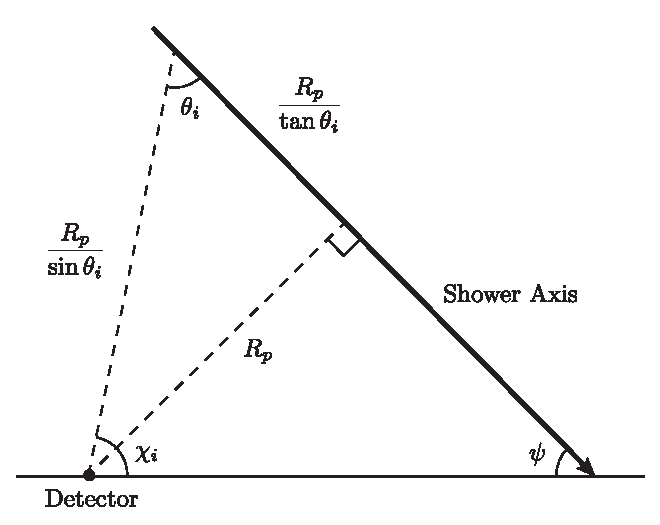
\includegraphics[width=0.8\textwidth]{MonoReconstruction}}
    \caption{The geometry of a monocular reconstruction. $\theta_i$ and $\chi_i$ change for each point along the shower axis, whereas $R_p$ and $\psi$ are properties of the entire shower.}
\end{figure}

Monocular experiments are desirable for their simplicity and lower cost, but as seen, come with compromises in data quality. We propose a technique which uses Cherenkov radiation to improve the accuracy of monocular reconstruction. Because Cherenkov radiation is collimated along the shower axis, most strikes the ground near the shower core, where some is reflected back into the detector. The reflection point lies along the shower axis, and can be used to reduce the number of parameters in the monocular fit from three to two. This reduction makes use of the following relationship:
\begin{equation} \label{eq:ckv_relation}
    R_p = d \sin(\psi + \alpha).
\end{equation}
$d$ is the distance from the detector to the ground reflection point, and $\alpha$ the angle of this point below the horizon. In this work, we investigate the feasibility of this Cherenkov-assisted reconstruction. Using simulations, we determine whether the Cherenkov reflection gives a strong signal and whether it can be used to improve accuracy.

\begin{figure}[!ht]
    \label{fig:hybridrecon}
    \centering
    \frame{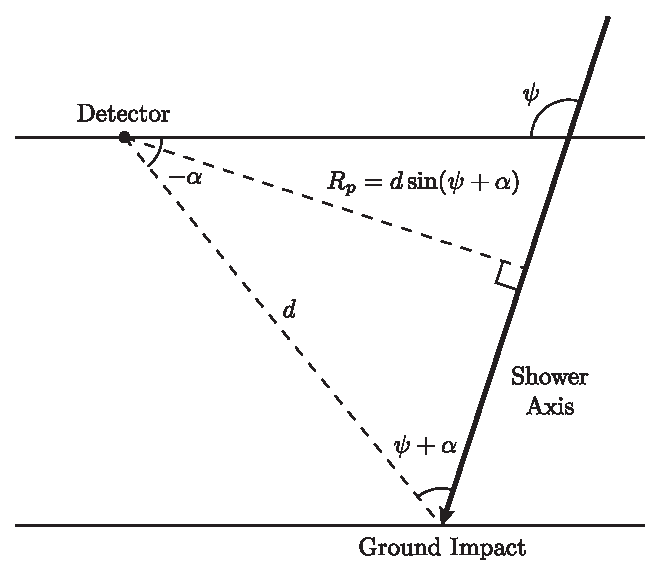
\includegraphics[width=0.8\textwidth]{CherenkovReconstruction}}
    \caption{The geometry of a Cherenkov-assisted reconstruction, showing the fixed relationship between $R_p$ and $\psi$.}
\end{figure}

The quality of the hybrid Cherenkov reconstruction depends considerably on the height $h$ of the detector above the ground. Assuming a Lambertian model of ground reflection, the amount of Cherenkov light seen is proportional to $\sin{\alpha}$. This means that the backscattering signal is nearly proportional to the detector height. In addition, the error in $d$ is inversely related to $h$ according to
\begin{equation} \label{eq:ground_err}
    \Delta d \approx \frac{d \Delta \alpha}{\sin{\alpha}} = \frac{d^2 \Delta \alpha}{h}.
\end{equation}
$\Delta \alpha$ is the angular size of a single pixel, and $\Delta d$ is the ground distance covered by a single pixel, equivalent to the error in $d$. The linear dependence on pixel size highlights the need for a high resolution detector. To achieve this, we use an f/1 Schmidt camera, which is a high-speed, wide-angle telescope with low spherical aberration. Both the focal surface and primary mirror are spherical, and in our simulation are given radii of \SI{1}{m} and \SI{2}{m}. A corrector plate is placed at the stop \cite{malacara2004optics}. As shown in Figure \ref{fig:schmidt}, the corrector has thick sections in the middle (a quadratic term), and near the edge (a quartic term). Because of the lens's large size, the decision was made to remove the central quadratic portion. This leaves a ring at the outside of the stop which could be assembled in slices. The detector height is varied throughout the simulation (see Section \ref{sec:results}).

\begin{figure}[!ht]
    \label{fig:schmidt}
    \centering
    \frame{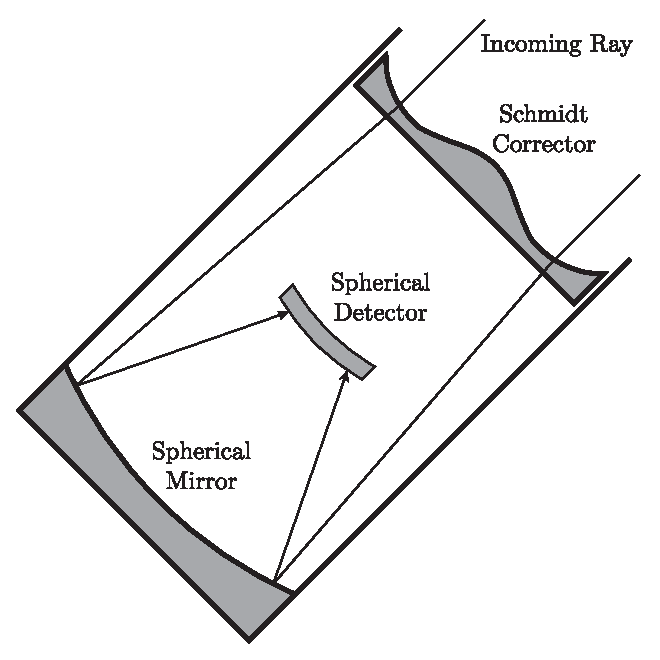
\includegraphics[width=0.8\textwidth]{SchmidtCamera}}
    \caption{A Schmidt camera. In this experiment, the thick inner portion of the corrector has been removed. The corrector deflects incoming rays to improve the camera's spherical symmetry.}
\end{figure}

\section{Summary of Simulation} \label{sec:sim_summary}

Simulating individual showers can give an idea of the typical appearance of the Cherenkov reflection and the quality of the hybrid reconstruction. More robust conclusions can be drawn from a Monte Carlo, which simulates a large number of representative showers. For all of these showers, a Cherenkov-assisted reconstruction is attempted and its accuracy is compared to the traditional method. Relative accuracies can be used to determine the range of parameters (e.g. angle or energy) in which the Cherenkov reconstruction gives an improvement. Each Monte Carlo iteration consists of three steps: the statistical generation of a shower, a simulation of its detection, and an attempt at reconstruction. The details of each of these steps are given in Section \ref{sec:methods}. When examining a specific shower energy and geometry the statistical generation step is eliminated. When probing the overall performance of the detector in a Monte Carlo, the generation-simulation-reconstruction process is repeated many times. Random shower energies are chosen from a power law and are used to determine Gaisser-Hillas parameters based on relations from Abuzayyad \cite{abuzayyad2000hires}. A direction and point of closest approach are randomly chosen. Using its direction, the shower is traced back from its closest approach to a starting point higher in the atmosphere.

From this starting point, the shower iterates through discrete steps of equal atmospheric thickness. At each step, the size of the shower is calculated from the Gaisser-Hillas profile and combined with parameterizations from Kakimoto and Nerling to obtain fluorescence and Cherenkov photon numbers \cite{gaisser1977profile,kakimoto1996yield,nerling2006electron}. These numbers are adjusted to account for the varying perspective and distance of the detector. Captured fluorescence photons are traced directly from the shower core to the detector. Cherenkov photons are given random directions around the shower axis, traced to their ground collision point, and reflected back into the detector. Both fluorescence and Cherenkov rays are traced through the detector optics to the pixel array, where they are binned and recorded.

This results in a three-dimensional histogram with a binned time series for each pixel on an x-y grid. If reconstruction were attempted immediately on this data set, it would usually be successful, regardless of the distance or brightness of the shower. Because this wouldn't give information about the real limits of the detector, background noise is first added to each time series. The noise in a particular bin is randomly sampled from a Poisson distribution. The mean noise level is then subtracted from the signal, and a bleeding algorithm is used to find chunks of non-noise signals. Triggering logic is applied to determine whether the track is sufficiently large and bright to attempt a reconstruction. If the detector is triggered, the shower-detector plane is fit and a standard monocular reconstruction is performed. A hybrid reconstruction is attempted if the Cherenkov reflection is sufficiently bright and within the field of view.